%!TEX root = ../../exa-ma-deliverables.tex
\section{2026 management and activity report}
\label{sec:management-year-4}

\noindent\emph{1 January--18 November 2026}

Exa-MA develops numerical methods and software for exascale
scientific computing within NumPEx. Its work covers discretisation,
solvers, model reduction and machine learning, inverse problems,
optimisation and uncertainty quantification. WP7 works with the
scientific teams to integrate their methods into software and test
them on common applications.

In 2026, the first demonstrators and mini-applications gave the
scientific and software teams common cases on which to test their
methods. At the June ANR review, Exa-MA set priorities for verification
and validation, GPU readiness, reproducible software releases and
benchmarks, and integration across NumPEx.

% Sources: October D0.2 draft by Jimmy James and Juliette Antonczak;
% 2026 coordination minutes; June ANR review slides and minutes;
% scientific WP contributions; Exa-MA website and dated partner announcements.

\subsection{The consortium in 2026}

Five beneficiary institutions receive ANR funding for Exa-MA. CNRS
and ten associated institutions contribute through laboratories and
research teams (\cref{fig:exama-consortium-2026}). The
\href{https://exa-ma.numpex.fr/consortium.html}{consortium register}
lists the participating teams.

Three projects involving consortium members started in 2026.
SAGE-HPC and DAiMOS joined the NumPEx programme, and JNL-G brings
IRMA and LNCMI together around the high-field magnet facility.
\Cref{tab:exama-ecosystem-2026} describes their links to Exa-MA.

\begin{figure}[!htb]
\centering
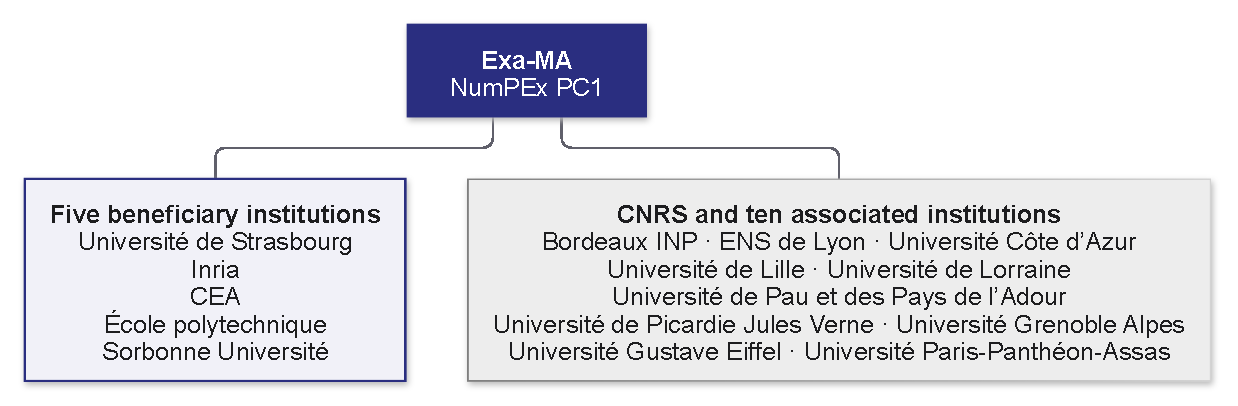
\includegraphics[width=\linewidth]{graphics/management/consortium-2026.pdf}
\caption{Exa-MA consortium in November 2026.}
\label{fig:exama-consortium-2026}
\end{figure}

\subsection{How the consortium works}

The project leads and project officers meet weekly, usually on
Tuesdays, for day-to-day decisions. The work package leads join them
every three weeks on Thursday mornings to review progress and agree
on joint work, recruitment and requests for computing time. The
project office keeps minutes and deliverables in the shared Drive.
By agreement with the ANR, Exa-MA operates without a steering committee.

The Exa-MA leads take part in the weekly Thursday evening meetings
with the NumPEx programme leadership (PC0) when the agenda calls for
their input.

\begin{figure}[!htb]
\centering
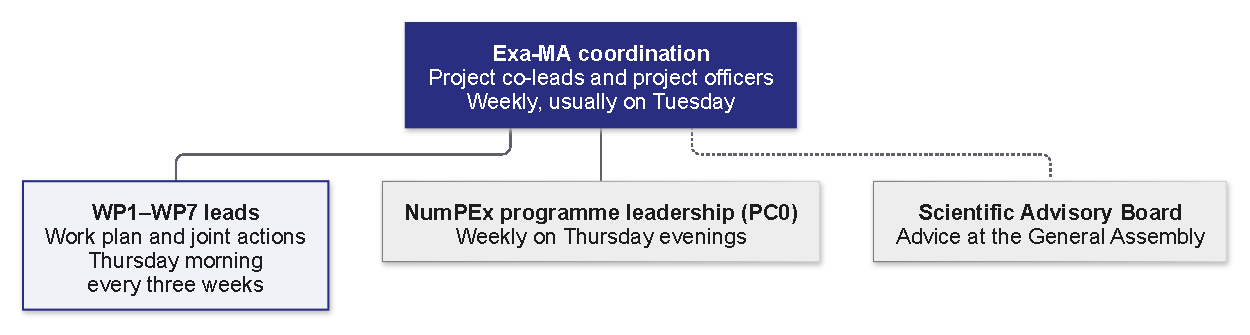
\includegraphics[width=\linewidth]{graphics/management/coordination-2026.pdf}
\caption{Working meetings and advisory and reporting relationships.}
\label{fig:exama-coordination-2026}
\end{figure}

The January General Assembly brought 65 participants from 24 institutions
to Aix-en-Provence and online. All seven work packages presented their
progress. The consortium discussed its research with the Scientific
Advisory Board and set aside working sessions on Feel++, Scimba,
Composyx and Uranie. The assembly programme and presentations are
available in the
\href{https://exa-ma.numpex.fr/news/2026/20260119-21-ag.html}{meeting report}.

% Exa-MA coordination minutes of 9 and 23 July and 3 September 2026.
% Exa-MA's July contribution is indexed in Zotero as exama2026agenticAIPosition.
After the May Operational Committee, Exa-MA prepared its contribution
on agentic AI for scientific computing and sent it to PC0 in July. It
proposed checking numerical results from simulations run by agents,
recording how they were obtained and evaluating agents on common
benchmarks. NumPEx announced the resulting
\href{https://numpex.org/4252/}{position paper} on 6 November.

\subsection{Scientific execution and computing resources}

At the May NumPEx Operational Committee, Exa-MA raised the need to
deploy the same benchmarks on different CPU and GPU systems. In WP3,
PETSc~3.25 added a CUDA backend for the HPDDM preconditioner. The June
discussion with the HPDDM team then identified two application cases
for follow-up, a discrete fracture network mini-app and a
thermo-mechanical benchmark. For heterogeneous diffusion with
Composyx, the additive Schwarz solver reached 88\% weak-scaling
efficiency on 32 Jean Zay nodes with NVIDIA V100 GPUs and 89\% on
128 Adastra nodes with AMD MI250X GPUs. Each series used its own
one-node reference.

WP5 tested a distributed optimiser with a variational quantum
eigensolver. The coupled workflow retained 60.98\% strong-scaling
efficiency on 1,000 LUMI-G nodes (8,000 GPUs).

The consortium submitted proposals to NumPEx in July for large runs on
the MI300A extension at CINES. The allocations under that call were
still pending on 18 November.

The June review identified the maturity of the WP4 and WP6 test cases
as a point to address. Both rely on methods developed across the
work packages, including discretisation and solvers. For WP4,
HiFiMagnet provides a case for estimating the parameters of a high-field
magnet from observations. The variational interface in Feel++ has
functional tests, and the application fiche specifies a benchmark for
parameter recovery. In the Ktirio Urban Building collaboration, WP6
implemented statistical processing for ensembles of urban-energy
simulations. WP6 has yet to validate that processing at application
scale, and the WP4 parameter-recovery benchmark remains planned.

In a separate collaboration between WP5 and WP6, tests with
Uranie's sensitivity indices improved optimisation on small problems.
Scaling the approach remains an open question.
\ifdefined\ExaMAStandaloneManagement\else
The work packages and application fiches give the test conditions and
results (\cref{chap:wp3,chap:wp4,chap:wp5,chap:wp6,chap:applications}).
\fi

\subsection{Deliverables, milestones and indicators}

After the June ANR review, PC0 asked the targeted projects for further
evidence on scientific results, risks, recruitment and collaborations.
Exa-MA contributed that material to the programme's midterm assessment
in September.

The October work plan called for updates to 20 deliverables. It covered
software releases (MS2), benchmarking (MS3), Level~1 demonstrators
(MS4) and mini-apps (MS5). The June schedule listed 14 June for MS4
and MS5. By September, the planned date for both was 14 October.
The 14 October submission was still outstanding on 18 November.

The October report counted 33 HAL records for 2026 through 14 October.
These included 11 journal articles, four conference papers, 17 preprints
or unpublished items, and one report. The project target over its
lifetime is more than 50 international peer-reviewed papers.

\subsection{Staffing and recruitment}

Erik Fabrizzi moved from an engineering post to a WP3 PhD at Sorbonne
Université. Maël Olivier, Bruno Latre and Quentin Bergez began doctoral
work at Inria. Robin Boëzennec and Edgar Jaber joined WP3 and WP6 as
postdoctoral researchers.
\Cref{tab:exama-staffing-2026} summarises appointments since the
start of the project.

\begin{table}[!htb]
\centering
\caption{Appointments wholly or partly funded by Exa-MA through 18 November 2026. The personnel register was updated on 5 November.}
\label{tab:exama-staffing-2026}
\small
\begin{tabular}{@{}lrrr@{}}
\toprule
\textbf{Appointment} & \textbf{Since launch} & \textbf{2026 starts} & \textbf{In post}\\
\midrule
Doctoral & 16 & 4 & 15\\
Postdoctoral & 7 & 2 & 3\\
Research engineering and project support & 8 & 0 & 5\\
\midrule
\textbf{Total} & \textbf{31} & \textbf{6} & \textbf{23}\\
\bottomrule
\end{tabular}
\end{table}

In May, École polytechnique agreed to redirect Exa-MA's share of a
planned PhD to a one-year engineering post on Uranie. École
polytechnique plans to recruit the engineer in the first quarter of
2027 to work with the CEA team in Saclay. WP5 redirected funding from a
planned doctorate to a postdoctoral position in optimisation and
reopened the search in September. The CEA--Inria PhD on block-structured
adaptive mesh refinement in WP1 was deferred to 2027.

\subsection{Financial follow-up}

At the March review, partners reported that higher doctoral salaries
had changed recruitment costs. Several also had difficulty obtaining
expenditure figures from their institutions. Exa-MA aims to review
partner expenditure every six months in coordination with PC0.

\subsection{External partnerships}

The ANR-funded \href{https://anr.fr/Project-ANR-25-CE46-1157}{JNL-G project}
reuses Exa-MA's multiphysics and model-reduction work in the digital
twin of the LNCMI high-field magnet facility in Grenoble. IRMA and
Cemosis are applying these methods in Feel++ and HiFiMagnet to model
the magnets together with their power supply and cooling systems.
The facility's measurements will guide validation of the models used
to study operating scenarios. JNL-G has its own funding and gives the
LNCMI and Exa-MA teams a setting in which to continue developing these methods.

Ktirio Urban Building brings Exa-MA's meshing and coupling work into
the HiDALGO2 urban-energy pilot and has been deployed on Jean Zay with
Exa-AToW. Cemosis is working with social housing providers, the
Eurométropole de Strasbourg and RTE, and is developing further
partnerships. These collaborations give the building and district-scale
models a use beyond the research project, for example to compare
renovation or energy scenarios with the partners.

% Thesis topic: Inria MACARON 2025 activity report, section 11.2.2.
\textbf{ENACT.} Exa-MA and the Grand Est AI cluster co-fund Vincent Italiano's
doctorate at the University of Strasbourg. He develops neural operators in WP2
to speed up forward wave simulations and the corresponding inverse calculations.

% Partnership updates from Hélène Barucq and Luc Giraud, 25 November 2026.
In passive imaging, correlations between recordings of ambient
waves carry information about the medium through which they travel.
Florian Faucher's ERC Starting Grant INCORWAVE develops nonlinear
inversion of the full correlation waveforms in the frequency domain.
It targets viscoelastic properties for subsurface monitoring and
three-dimensional flows for studies of solar convection. The team
studies how to introduce data, frequencies and unknown parameters
in stages to improve the convexity of the misfit and the resolution
when prior information is limited. The need to repeat large wave
simulations connects the inverse methods in WP4 with optimisation
in WP5.
\href{https://cordis.europa.eu/project/id/101116288}{INCORWAVE project summary}.

Through the ANR--DFG project BUTTERFLY, Inria Makutu and the
Göttingen helioseismology group, including the Max Planck Institute
for Solar System Research, worked with the MUMPS team on a 3D solver
for time-harmonic oscillations throughout the Sun and its
photosphere. Hawen adapts the polynomial order to the local
wavelength and eliminates element-interior unknowns before the
global solve. The team validated the solver against an axisymmetric
reference and used it to study how active regions and convection
affect wave propagation. The October 2026 paper describes systems
of up to 376 million global unknowns and reports a factorisation of
310 million on 100 Adastra nodes. In a 50-node comparison, block
low-rank factors and mixed-precision storage reduced factorisation
memory from 12.4 to 6.7~TB. The results show how WP1 discretisation
and the Exa-SofT (PC2) sparse solver complement each other at scale.
\href{https://link.springer.com/article/10.1007/s10915-026-03489-0}{Journal article} and
\href{https://arxiv.org/abs/2511.22530v1}{open preprint (Section 5.4)}.

\Cref{fig:exama-ecosystem-2026,tab:exama-ecosystem-2026} summarise
the wider partnership network.

\begin{figure}[!htb]
\centering
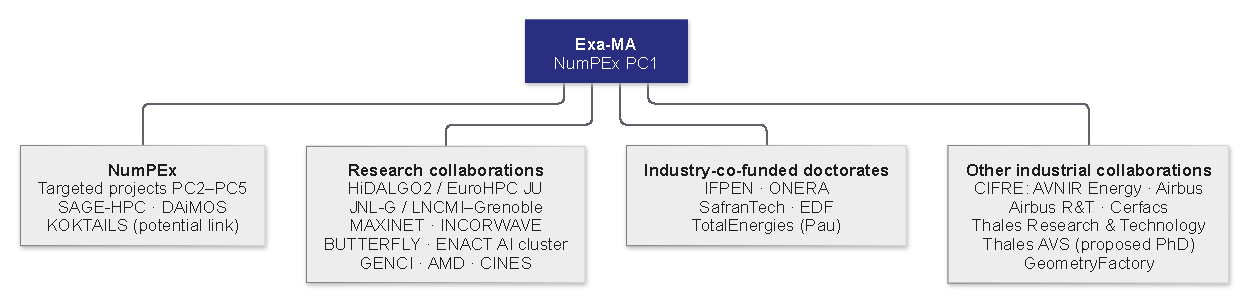
\includegraphics[width=\linewidth]{graphics/management/ecosystem-2026.pdf}
\caption{Selected projects and organisations linked to Exa-MA in November 2026.}
\label{fig:exama-ecosystem-2026}
\end{figure}

%!TEX root = ../../exa-ma-deliverables.tex
% The June ANR review deck (slides.exa-ma.anr.20260611/content.typ and
% assets/exa-ma-ecosystem-links.svg) covers 2025 and early 2026. The rows
% below retain those dates and add evidence from 2026 where available.
\begingroup
\small
\setlength{\tabcolsep}{4pt}
\renewcommand{\arraystretch}{1.12}
\begin{longtable}{@{}
  >{\raggedright\arraybackslash}p{0.225\textwidth}
  >{\raggedright\arraybackslash}p{0.155\textwidth}
  >{\raggedright\arraybackslash}p{0.57\textwidth}@{}}
\caption{Exa-MA research collaborations and related projects, November 2026.}
\label{tab:exama-ecosystem-2026}\\
\toprule
\textbf{Project or institution} & \textbf{Status} & \textbf{Work and links to Exa-MA}\\
\midrule
\endfirsthead
\toprule
\textbf{Project or institution} & \textbf{Status} & \textbf{Work and links to Exa-MA}\\
\midrule
\endhead
\midrule
\multicolumn{3}{r@{}}{\emph{Continued on next page}}\\
\endfoot
\bottomrule
\endlastfoot

\multicolumn{3}{@{}l@{}}{\textbf{\href{https://numpex.org/projects/}{NumPEx targeted projects}}}\\*
PC2 --- Exa-SofT & Software collaboration &
WP3 works on composable linear algebra with Composyx. WP1 has
explored StarPU for FunTiDES. \href{https://exa-ma.numpex.fr/workpackages/wp7.html}{WP7
software integration}.\\[1pt]

PC3 --- Exa-DoST & Scientific collaboration &
Adaptive-mesh I/O and coupling Scimba with the GYSELA plasma
code. Exa-DoST also reports joint work on turbulence models. \href{https://numpex.org/wp-content/uploads/sites/6/2025/12/2025-11-05-01-NumPEx-and-Exa-DoST-Overview-Gabriel.pdf}{Exa-DoST
assembly overview}.\\[1pt]

PC4 --- Exa-AToW & Workflow collaboration &
The June ANR review records PC4's first deployment of Ktirio Urban
Building on Jean Zay.\\[1pt]

PC5 --- Exa-DI & Co-design &
Joint work on high-order discretisation, adaptive and unstructured
meshes, and application demonstrators. \href{https://numpex.org/exadi-development-and-integration/}{Exa-DI
programme and annual meeting}.\\

\addlinespace
\multicolumn{3}{@{}l@{}}{\textbf{\href{https://numpex.org/projects-call-2025/}{Projects funded through the 2025 NumPEx call}}}\\*
SAGE-HPC & Started in 2026 &
AI for HPC, focused on multifidelity optimisation. Inria and
Cemosis/IRMA share teams with Exa-MA. \href{https://numpex.org/wp-content/uploads/sites/6/2026/02/2026-01-21-1-SageHPC.pdf}{Assembly
slides}.\\[1pt]

DAiMOS & Started in 2026 &
HPC for AI, focused on distributed training. IRIT--Toulouse INP,
Inria Bordeaux, Sorbonne Université and Météo-France form the
consortium. \href{https://numpex.org/wp-content/uploads/sites/6/2026/02/2026-01-21-2-DAIMOS.pdf}{Assembly
slides}.\\[1pt]

KOKTAILS & Potential link &
GPU portability with Kokkos, including unstructured meshes. IFPEN
and Inria are involved.\\

\addlinespace
\multicolumn{3}{@{}l@{}}{\textbf{Research programmes and facilities}}\\*
HiDALGO2 / EuroHPC JU & Joint pilot and training &
Université de Strasbourg/Cemosis link WP1 and WP7 to the \href{https://www.hidalgo2.eu/urban-building-model/}{Ktirio Urban
Building pilot}. The teams and NCC France held a
\href{https://exa-ma.numpex.fr/training.html}{joint webinar on 12 January 2026}.\\[1pt]

JNL-G / LNCMI--Grenoble & Started in 2026 &
The LNCMI--IRMA digital twin reuses Exa-MA multiphysics and
model-reduction methods in Feel++ and HiFiMagnet.
\href{https://anr.fr/Project-ANR-25-CE46-1157}{ANR project summary}.\\[1pt]

% Funding shares from Exa-MA's 2025 ANR return, WP2 staffing.
\href{https://cluster-ia-enact.ai/}{ENACT AI cluster} & Co-funded WP2 PhD &
Exa-MA and the Grand Est AI cluster each fund half of Vincent
Italiano's doctoral contract.\\[1pt]

GENCI, AMD and CINES & Technical exchanges &
Exa-MA proposed three pilot topics with WP1, WP3 and WP5 at the
\href{https://exa-ma.numpex.fr/news/archive.html}{February workshop
in Saclay}.\\

\end{longtable}
\endgroup


\subsection{Industrial partnerships}

\Cref{tab:exama-industrial-phds-2026} lists the four doctorates
co-funded by Exa-MA and its industrial partners alongside other
industrial collaborations.

%!TEX root = ../../exa-ma-deliverables.tex
% Sources: external partners workshop and January 2026 General Assembly slides,
% Exa-MA partner register, and the June 2026 ANR review.
\begin{table}[!htb]
\centering
\caption{Doctoral projects co-funded by Exa-MA and industrial partners.}
\label{tab:exama-industrial-phds-2026}
\small
\setlength{\tabcolsep}{4pt}
\renewcommand{\arraystretch}{1.12}
\begin{tabular}{@{}
  >{\raggedright\arraybackslash}p{0.285\linewidth}
  >{\raggedright\arraybackslash}p{0.255\linewidth}
  >{\raggedright\arraybackslash}p{0.415\linewidth}@{}}
\toprule
\textbf{Partners and host team} & \textbf{Funding} & \textbf{Research}\\
\midrule
IFPEN and ONERA \newline Inria Alpines &
50\% Exa-MA, 25\% IFPEN and 25\% ONERA &
Learning-based solvers and preconditioners for sparse linear systems.\\[2pt]
ONERA and Safran \newline École polytechnique &
50\% Exa-MA, 50\% ONERA and Safran jointly &
High-order adaptive time coupling for multiphysics simulations.\\[2pt]
EDF \newline Sorbonne Université &
Exa-MA and EDF &
Scalable preconditioners for nonsymmetric saddle-point problems in WP3.\\[2pt]
TotalEnergies \newline Inria Makutu, Pau &
50\% Exa-MA, 50\% TotalEnergies &
Modular HPC software for solving PDEs, including AI-assisted design of numerical schemes.\\
\bottomrule
\end{tabular}
\end{table}


% Funding applications and follow-up for the four co-funded doctorates:
% IFPEN--ONERA: https://drive.google.com/file/d/1p_qcfyeSpq4WGzIYy4E6LV_zAqWkt0vQ/view
% ONERA--SafranTech: https://drive.google.com/file/d/1VhROImSQyZ_9KCINXJFVHqVnGm-tKm-w/view
% EDF: https://drive.google.com/file/d/1wDycXWxD9R_5YHLuf9S7y8PC85FdZLau/view
% TotalEnergies: https://app.doctorat.gouv.fr/proposition?id=15465
% Consortium follow-up: https://docs.google.com/document/d/1jpxB9UWpdkh3dGlcHHHV7YGBVX4xEY1H5xQg1-SKmNk/edit
\textbf{IFPEN and ONERA.}
Graph neural networks supply preconditioners and initial guesses for Krylov
solvers. The project targets large sparse systems from subsurface hydrogen
and CO$_2$ storage at IFPEN and compressible turbulent flow at ONERA (WP2 and WP3).

\textbf{ONERA and SafranTech.}
High-order time coupling adapts when multiphysics solvers exchange data.
The project targets integration into CWIPI and testing on a fire-safety
case where a reacting flow heats and degrades a solid material (WP1 and WP3).

\textbf{EDF.}
The project develops scalable preconditioners for nonsymmetric saddle-point
systems in fluid and solid mechanics. It uses HPDDM and PETSc with EDF test
cases in \texttt{code\_saturne} and \texttt{code\_aster} (WP3 and WP7).

\textbf{TotalEnergies.}
Reduced models built from spectral-element simulations aim to accelerate elastic
full-waveform inversion. The project estimates errors from model reduction and
from seismic shot sampling separately to guide stochastic optimisation.

\begin{samepage}
\subsubsection*{Other industrial collaborations}

Hanna Chetouane began her CIFRE doctorate with AVNIR Energy and
Cemosis in October. The project aims to monitor thin industrial
structures by inferring defects from their vibration and acoustic
response. It will combine experimental measurements with high-order
finite-element models in Feel++ that account for the interaction
between the structure and the surrounding fluid. The mathematical
work draws on multiphysics coupling in WP1, fast solvers for CPUs
and GPUs in WP3 and inverse methods in WP4. The CIFRE provides
research capacity in kind to Exa-MA.
\href{https://www.cemosis.fr/en/news/cifre-avnir-energy/}{AVNIR Energy CIFRE project}.
\end{samepage}

Simulating aircraft noise requires fine finite-element meshes where
the flow varies sharply, for instance in the engine jet.
In her CIFRE doctorate with Airbus and Inria Makutu, Andréa Lagardère
uses generalised plane waves that approximate the wave equation
with the local flow coefficients in each element. These
quasi-Trefftz basis functions allow larger elements and fewer
unknowns in the discontinuous Galerkin model. The team coupled the
method in the frequency domain to a boundary element solver for
the surrounding region, where the flow is taken to be uniform.
It integrated the coupling into Airbus's HPC code Actipole and
validated it on an industrial case, linking WP1's discretisation
work to aircraft noise simulation.
\href{https://trefftz2026.univie.ac.at/}{September 2026 workshop}.

Concace (Inria, Airbus Central R\&T and Cerfacs) develops neural
preconditioners for simulating aircraft noise near urban airports.
Self-supervised training uses equation residuals in single precision
(32 bit). The network preconditions a flexible GMRES solve carried
out in double precision (64 bit). On the two-dimensional Helmholtz reference
tests, the solver reached a backward error of $10^{-10}$ in fewer
than 20 iterations. The team reused a network trained on systems
of 4\,096 unknowns on problems with up to 262\,144 unknowns and tested
it with sound speeds outside the training range. The work links
learning in WP2 to solvers in WP3. It relies primarily on team
resources, with support from ANR Maturation.
\href{https://arxiv.org/abs/2610.16542}{2026 study}.

\subsection{Training and exchanges between teams}

The June MAJSC workshop in Strasbourg combined lectures on automatic
differentiation with practical work in JAX. The hands-on material
covers differentiable PDE solvers, neural methods and optimal control.
Four software sessions that month gave the WP teams direct access to
the developers of HPDDM/PETSc, TRUST, FreeFEM++ and Samurai. The
discussions concerned concrete engineering questions, from moving
preconditioners to GPUs to choosing data structures for adaptive meshes.
The project officers set up shared GitHub boards for the frameworks
to record actions by work package and institution and follow the
preparation of mini-applications. The slides and recordings are linked
in \cref{tab:exama-news-2026}.
\ifdefined\ExaMAStandaloneManagement
The \href{https://exa-ma.numpex.fr/deliverables.html}{deliverables
collection} includes D7.3, the training report.
\else
\Cref{chap:training} gives the courses and links to the training material.
\fi

\subsection{Website and public communication}

Exa-MA launched its \href{https://exa-ma.numpex.fr/}{website} in 2024,
following that year's General Assembly. The January 2026 update expanded
the work package pages and software catalogue, linking teams to their
software, application cases and publications. The site also hosts team
and partner directories, versioned deliverables, training resources and
an event archive with programmes, slides and recordings.

Antora builds the site from AsciiDoc pages. The event register supplies
the lists on the home page, the news page and the archive. A daily build
refreshes the
\href{https://exa-ma.numpex.fr/publications-hal.html}{publication list}
from HAL using the funding reference \texttt{ANR-22-EXNU-0002}. The page
groups HAL records by year. In October, Exa-MA proposed adding
publications supported by in-kind contributions.

Exa-MA no longer has a dedicated communications contact. PC0 has recruited
a communications officer to set up exchanges between the NumPEx programme
and its targeted projects, including Exa-MA. \Cref{tab:exama-news-2026}
brings together announcements and events from the Exa-MA
\href{https://exa-ma.numpex.fr/news/archive.html}{news archive} and the
NumPEx programme.

%!TEX root = ../../exa-ma-deliverables.tex
% Sources: Exa-MA news archive, NumPEx announcements and event programmes through 18 November 2026.
\begingroup
\small
\setlength{\tabcolsep}{4pt}
\setlength{\LTpre}{6pt}
\renewcommand{\arraystretch}{1.04}
\begin{longtable}{@{}%
  >{\raggedright\arraybackslash}p{0.16\textwidth}
  >{\raggedright\arraybackslash}p{0.30\textwidth}
  >{\raggedright\arraybackslash}p{0.49\textwidth}@{}}
\caption{Selected Exa-MA and NumPEx announcements and events in 2026.}
\label{tab:exama-news-2026}\\
\toprule
\textbf{Date} & \textbf{Announcement or event} & \textbf{Exa-MA contribution}\\
\midrule
\endfirsthead
\toprule
\textbf{Date} & \textbf{Announcement or event} & \textbf{Exa-MA contribution}\\
\midrule
\endhead
\midrule
\multicolumn{3}{r@{}}{\emph{Continued on next page}}\\
\endfoot
\bottomrule
\endlastfoot
12 January &
\href{https://www.hidalgo2.eu/webinar-on-global-challenges-and-built-environments-discover-4-hpc-applications-use-cases/}{HiDALGO2 and NCC France webinar} &
WP1 and WP7 presented Ktirio Urban Building for city-scale energy simulation.\\
14 January &
\href{https://exa-ma.numpex.fr/news/archive.html}{Website update} &
Expanded work package pages and software catalogue, with links to
reports and publications.\\
19--21 January &
\href{https://exa-ma.numpex.fr/news/2026/20260119-21-ag.html}{General Assembly, Aix-en-Provence} &
WP reviews, software sessions and a discussion with the Scientific
Advisory Board. Daria Hrebenshchykova became Exa-MA's YoungPEx representative.\\
2--5 February &
\href{https://exa-ma.numpex.fr/news/2026/20260202-05-transnumeriques.html}{Trans-Numériques, Rennes} &
Exa-MA contributed sessions on AI and HPC and on the software
ecosystem.\\
18--19 February &
\href{https://exa-ma.numpex.fr/news/archive.html}{AMD and NumPEx technical meeting, Saclay} &
WP1, WP3 and WP5 proposed topics for joint pilot studies with AMD.\\
7 May &
\href{https://exa-ma.numpex.fr/news/archive.html}{NumPEx Operational Committee, Paris} &
Exa-MA raised the deployment of common benchmarks on heterogeneous
systems.\\
26--28 May &
\href{https://aissai-hace.sciencesconf.org/?lang=en}{AISSAI--NumPEx HACE workshop, Toulouse} &
Emmanuel Franck (WP2) chaired the session on AI-based surrogates for PDEs.\\
8--12 June &
\href{https://majsc2026.pages.math.unistra.fr/program.html}{MAJSC workshop, Strasbourg} &
Lectures and practical sessions on JAX and automatic differentiation
for scientific computing.\\
11 June &
\href{https://exa-ma.numpex.fr/news/archive.html}{NumPEx annual review with the ANR} &
Exa-MA presented scientific results, collaboration and progress on the
project milestones.\\
22--26 June &
\href{https://exa-ma.numpex.fr/news/2026/20260622-hpddm-petsc-framework-webinar.html}{HPDDM/PETSc} (22),
\href{https://exa-ma.numpex.fr/news/2026/20260623-trust-framework-webinar.html}{TRUST} (23),
\href{https://exa-ma.numpex.fr/news/2026/20260625-freefem-framework-webinar.html}{FreeFEM++} (25) and
\href{https://exa-ma.numpex.fr/news/2026/20260626-samurai-framework-webinar.html}{Samurai} (26) &
Four software sessions on GPU preconditioning, Kokkos porting,
finite-element solver interfaces and adaptive mesh refinement.\\
7--9 September &
\href{https://aissai-jaxhack.sciencesconf.org/}{AISSAI--NumPEx JAX hackathon, IDRIS} &
Emmanuel Franck (WP2) taught an introductory JAX session for scientific computing.\\
6 November &
\href{https://numpex.org/4252/}{NumPEx position paper on agentic AI for science} &
Exa-MA contributed proposals on numerical validation, reproducibility
and benchmarking.\\
17 November &
\href{https://exa-ma.numpex.fr/news/2026/20261117-fem.html}{Forum Entreprises \& Mathématiques, Paris} &
Christophe Prud'homme moderated the HPC--AI panel on skills and careers.
Emmanuel Franck was a panellist.\\
\end{longtable}
\endgroup

